\chapter{Bildverarbeitung} \label{chap:Bildverarbeitung}

Die Bildverarbeitung besteht im Wesentlichen aus der Generierung von einzelnen Videoframes im RGB565 – Bitmap Format, welche optisch den Anforderungen aus Kapitel \ref{FunkAnf} entsprechen müssen. Die einzelnen Videoframes werden von der Schnittstelle \textit{IFrameProvider} empfangen und nach der Verarbeitung an die Schnittstelle \textit{FrameViewer} zur Darstellung auf dem Display des Smartphones weitergereicht.
\\
\\
Im ersten Ansatz, der verfolgt wurde, war eine Konvertierung notwendig als Vorverarbeitung der einzelnen Frames in den RGB Farbraum (siehe Kapitel \ref{YUV_RGBKonvert}). Diese Vorverarbeitung wurde im späteren Verlauf überflüssig, da das Übertragungsformat der Videoframes aufgrund der in Kapitel \ref{PerfFunk} genannten Gründen geändert wurde. Der Vollständigkeit halber wird die eben genannte Konvertierung hier trotzdem erläutert.
\\
\\
Es wurde davon ausgegangen, dass die Schnittstelle \textit{IFrameProcessor} Byte-Streams im Format NV12 (YUV420) erhält, welche zur weiteren Verarbeitung zunächst in den RGB Farbraum überführt werden mussten, um dann als \textit{Bitmap}-Objekte weiterverarbeitet werden zu können. Die NV12 Byte-Streams liegen im YUV-Farbmodell (siehe Kapitel \ref{YUV_RGBKonvert}) vor. 
\\
\\
Die Methode \textit{convertNv12ToBmp(...)} (siehe Listing \ref{lst:NV12_to_BMP}) nimmt ein eindimensionales Byte-Array, welches ein Frame im NV12-Format repräsentiert, entgegen. Die Methode benötigt zusätzlich noch die Höhe und Breite des Frames in Pixeln, um die Positionen der für ein Ausgabepixel relevanten Y, U und V Werte im Array bestimmen zu können. Innerhalb der for-Schleife werden für jedes einzelne Ergebnis-Pixel die in Kapitel \ref{YUV} Luminanz- und Chrominanz-Werte aus dem Array ermittelt und an die Methode \textit{convertYUVtoRGB(...)} übergeben. Ergebnis dieser Methode ist ein Array aus Integer-Werten, welche jeweils die Farbe eines Pixels repräsentieren. Mit Hilfe dieses Arrays kann anschließend mit der Methode \textit{createBitmap(...)} der Klasse \textit{Bitmap} aus dem Android SDK ein Bitmap-Objekt erzeugt werden. 
\clearpage

\begin{lstlisting}[caption=Methode \textit{convertNv12ToBmp()} zur Überführung eines Byte-Arrays im NV12-Format in ein Bitmap-Objekt, label=lst:NV12_to_BMP, language=Java]
public interface INalUExtractor
{
    private static int[] convertNv12ToBmp(byte[] rawFrame, int width, int height) {
        int size = width*height;
        int offset = size;
        int[] pixels = new int[size];
        int u, v, y1, y2, y3, y4;


        for(int i=0, k=0; i < size; i+=2, k+=2) {
            y1 = rawFrame[i  ]&0xff;
            y2 = rawFrame[i+1]&0xff;
            y3 = rawFrame[width+i  ]&0xff;
            y4 = rawFrame[width+i+1]&0xff;

            u = rawFrame[offset+k  ]&0xff;
            v = rawFrame[offset+k+1]&0xff;
            u = u-128;
            v = v-128;

            pixels[i  ] = convertYUVtoRGB(y1, u, v);
            pixels[i+1] = convertYUVtoRGB(y2, u, v);
            pixels[width+i  ] = convertYUVtoRGB(y3, u, v);
            pixels[width+i+1] = convertYUVtoRGB(y4, u, v);

            if (i!=0 && (i+2)%width==0)
                i+=width;

            log.info("i: " + i);
        }

        return pixels;
    }
}
\end{lstlisting}

~\\
Die in Listing \ref{lst:YUV_to_RGB} gezeigte Methode \textit{convertYUVtoRGB(...)} übernimmt gemäß der Formeln aus Kapitel \ref{YUV_RGBKonvert} die Berechnung der R, G und B Werte eines Pixels des Ergebnis-Frames. Aus diesen drei Werten wird anschließend ein Integer berechnet, welcher dann allein die Farbe des Pixels repräsentiert.
\clearpage

\begin{lstlisting}[caption=Methode \textit{convertYUVtoRGB(...)} zur Umrechnung eines Pixels aus dem YUV-Farbraum in den RGB-Farbraum, label=lst:YUV_to_RGB, language=Java]
private static int convertYUVtoRGB(int y, int u, int v) {
        int r,g,b;


        r = y + (int)(1.402f*v);
        g = y - (int)(0.344f*u +0.714f*v);
        b = y + (int)(1.772f*u);
        r = r>255? 255 : r<0 ? 0 : r;
        g = g>255? 255 : g<0 ? 0 : g;
        b = b>255? 255 : b<0 ? 0 : b;

        return 0xff000000 | (r<<16) | (g<<8) | b;
    }
\end{lstlisting}

~\\
Wie bereits weiter oben erwähnt, wurde die eben beschriebene Konvertierung obsolet, da der \textit{IFrameProcessor}-Schnittstelle aus in Kapitel \ref{PerfFunk} genannten Gründen direkt die einzelnen Videoframes als \textit{Bitmap}-Objekte im RGB565 Format geliefert bekommt. Diese Frames beinhalten das unveränderte Bildmaterial des Ultraschallgeräts, wie es auf dessen Monitor angezeigt wird. Da nicht alle Komponenten des Bildes relevant für die Erfüllung der in Kapitel \ref{FunkAnf} beschriebenen Anforderungen sind, erfolgt zunächst eine Auswahl der relevanten Ausschnitte des Bildes, um diese anschließend gemäß der Konzeptzeichnung (siehe Abbildung \ref{fig:Ausgabeframe}) neu anzuordnen. 

\begin{figure}[h]
	\centering
	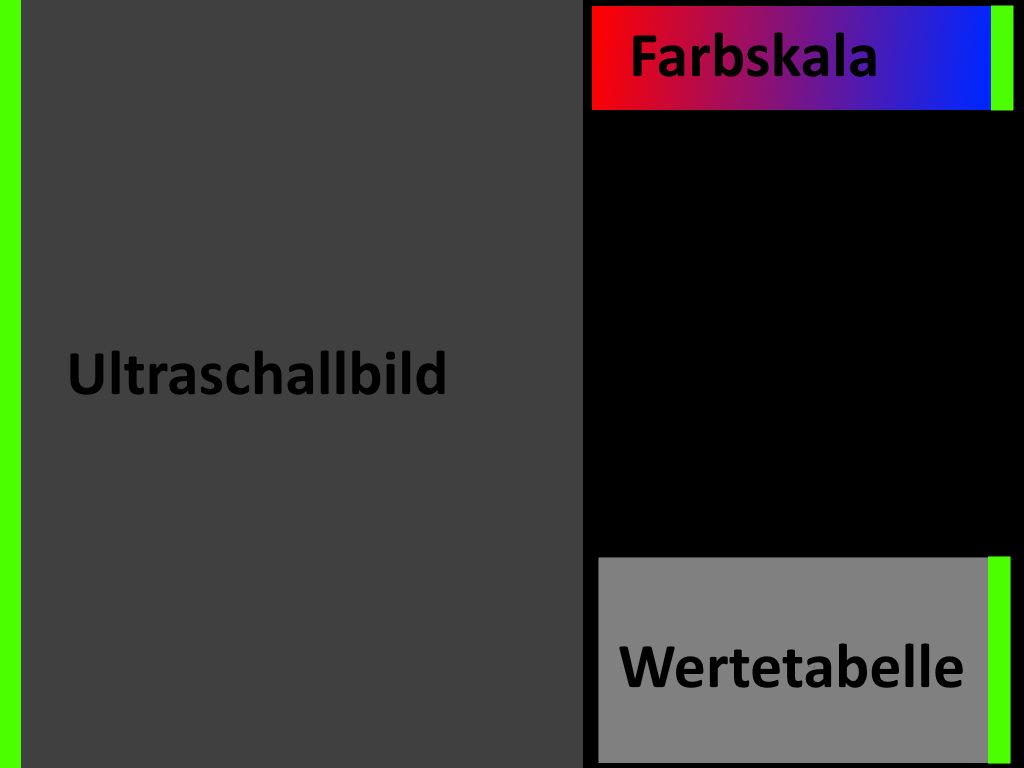
\includegraphics[width=0.5\textwidth]{Bilder/Bildverarbeitung/Konzept_Endframe.PNG}
	\caption{Konzeptzeichnung Ausgabeframe}
	\label{fig:Ausgabeframe}
\end{figure}

~\\
Der grüne Rand der einzelnen Komponenten in der Konzeptzeichnung (Abbildung \ref{fig:Ausgabeframe}) zeigt den oberen Rand dieser im Originalbild. Das Ultraschallbild wird also entsprechend um 270° und die Farbskala und Wertetabelle um 90° gedreht dargestellt. Zu beachten ist, dass die Ausgabeframes auf dem Display des Smartphones vertikal mit dem Ultraschallbild zum Teilerspiegel zeigend dargestellt werden. Diese Anordnung ermöglicht eine Darstellung des Ultraschallbildes in der Breite des Schallkopfes und eine leichte Lesbarkeit der Wertetabelle und Farbskala.
\\
\\
Listing \ref{lst:extractUltrasonicScan} zeigt beispielhaft für das Ausschneiden der für das Ausgabebild relevanten Komponenten die Methode \textit{extractUltrasonicScan()}. Da sich das Ultraschallbild an fester Stelle im Originalvideo befindet, konnten feste Werte für dieses ermittelt und in der Methode verwendet werden. Aus dem ausgeschnittenen Rechteck wird dann ein \textit{Bitmap}-Objekt der Größe dessen generiert.

\begin{lstlisting}[caption=Methode \textit{extractUltrasonicScan()} zum Ausschneiden des Ultraschallbildbereichs aus dem Originalframe, label=lst:extractUltrasonicScan, language=Java]
private Bitmap extractUltrasonicScan () {
        Rect UltrasonicScanRegion = new Rect(298, 60, 691, 507);
        Bitmap UltrasonicScan = Bitmap.createBitmap(source, 298, 60,
                UltrasonicScanRegion.width(), UltrasonicScanRegion.height());

        return UltrasonicScan;
    }
\end{lstlisting}

~\\
Die nachfolgend abgebildete Methode \textit{buildFinalFrame()} (Listing \ref{lst:buildFinalFrame}) baut die einzelnen Komponenten, welche mit den Methoden \textit{extractUltrasonicScan()}, \textit{extractColorScale()} und \textit{extractValues()} extrahiert werden, zu einem Frame gemäß Abbildung \ref{fig:Ausgabeframe} zusammen. Hierzu werden zunächst zwei Rotationsmatrizen erzeugt, eine die eine Rotation um 270° und eine, die eine Rotation um 90° vollzieht. Mit Hilfe dieser Matrizen werden anschließend die drei Komponenten rotiert und in neuen \textit{Bitmap}-Objekten zwischengespeichert. Für das \textit{Bitmap}-Objekt \textit{result} werden die Konfigurationen des Quellobjekts übernommen. Anschließend wird es einem \textit{Canvas}-Objekt übergeben, auf dem dann die drei vorverarbeiteten Komponenten angeordnet werden. Hierfür wird noch eine Skalierung des Ultraschallbildobjekts vorgenommen, sodass dies die volle Höhe des Ausgabeframes als Breite beansprucht (siehe Abbildung \ref{fig:Ausgabeframe}).
\clearpage

\begin{lstlisting}[caption=Methode zum Zusammenstellen des Ausgabeframes, label=lst:buildFinalFrame, language=Java]
private Bitmap buildFinalFrame() {

        Bitmap firstImage = extractUltrasonicScan();
        Bitmap secondImage = extractColorScale();
        Bitmap thirdImage = extractValues();

        Matrix matrix = new Matrix();
        matrix.postRotate(270);

        Matrix m180 = new Matrix();
        m180.postRotate(90);

        Bitmap rotColorScale = Bitmap.createBitmap(secondImage, 0, 0,
                secondImage.getWidth(), secondImage.getHeight(), m180, true);
        Bitmap rotUltraSonicScan = Bitmap.createBitmap(firstImage, 0, 0,
                firstImage.getWidth(), firstImage.getHeight(), matrix, true);
        Bitmap rotValues = Bitmap.createBitmap(thirdImage, 0, 0,
                thirdImage.getWidth(), thirdImage.getHeight(), m180, true);

        Bitmap result = Bitmap.createBitmap(source.getWidth(), source.getHeight(),
                source.getConfig());
        Canvas canvas = new Canvas(result);

        Rect UltrasonicScanRegion = new Rect(0, 0, rotUltraSonicScan.getWidth(),
                rotUltraSonicScan.getHeight());
        Rect scaledUltrasonicRect = new Rect(0, 0, 873, 768);

        canvas.drawBitmap(rotUltraSonicScan, UltrasonicScanRegion,
                scaledUltrasonicRect, null);
        canvas.drawBitmap(rotColorScale, 630, 50, null);
        canvas.drawBitmap(rotValues, 630, 600, null);

        return result;
    }
\end{lstlisting}

~\\
Um zu vermeiden, dass bereits vor dem Schallen Frames der Auswahlfenster der SonoScape-Software verarbeitet und zur Anzeige auf das Display des Smartphones gebracht werden, wurde eine Methode geschrieben, welche überprüft ob die SonoScape-Software in den Schall-Modus gewechselt ist. Diese Überprüfung geschieht simpel über einen Farbvergleich von Pixeln. Es wurden Pixel an Positionen gewählt, bei denen davon auszugehen ist, dass ihre Farbe schwarz ist, solange sich die SonoScape-Software im Schall-Modus befindet.  
\\
\\
Zum isolierten Testen der Bildverarbeitung im \textit{IFrameProcessor} wurde eine Testklasse \textit{FrameProcessorImplTest} geschrieben, welche einzelne Testframes als BIN-Dateien, die zuvor mit dem Ultraschallgerät aufgenommen wurden, aus dem SD-Kartenspeicher des Smartphones (oder des Emulators) lädt und diese zum Verarbeiten an die \textit{IFrameProcessor}-Schnittstelle weiterleitet. Für die Evaluierung der Bildverarbeitung wurden die bearbeiteten Frames anschließend als PNG-Dateien wieder in den SD-Kartenspeicher geschrieben. 
\\
Um Testdateien in den SD-Kartenspeicher des AndroidStudio-Emulators (siehe Kapitel \ref{Android}) zu schreiben, bzw. sie aus diesem auszulesen, wurden folgende Befehle über die AndroidStudio-Konsole eingegeben:
\\
\\
Schreiben: \textit{adb push path/yourfile.xxx /sdcard/yourfile.xxx}
\\
Lesen: \textit{adb pull /sdcard/yourfile.xxx /path/yourfile.xxx}
\\
\\
Damit die \textit{IFrameProcessor}-Schnittstelle überhaupt angesprochen werden kann, musste für die Testklasse die Methode \textit{loadRGBFile()} (Listing \ref{lst:BIN_to_Bitmap}) implementiert werden, die aus einer BIN-Datei, die ein Frame im RGB565-Format enthält, ausliest und in ein \textit{Bitmap}-Objekt schreibt. 

\clearpage
\begin{lstlisting}[caption=Methode \textit{loadRGBFile()} zum Einlesen einer BIN-Datei im RGB565-Format zu Testzwecken, label=lst:BIN_to_Bitmap, language=Java]
public Bitmap loadRGBFile() throws FileNotFoundException{

        Bitmap b = Bitmap.createBitmap(1024, 768, Bitmap.Config.RGB_565);
        byte[] bytes = null;
        File rgb;
        File sdDir = Environment.getExternalStorageDirectory();
        rgb = new File(sdDir, "testfileRGB.bin");

        if(rgb.exists()) {

            FileInputStream fis = new FileInputStream(rgb);
            ByteArrayOutputStream bos = new ByteArrayOutputStream();
            byte[] buf = new byte[1024*768*2];
            try {
                for (int readNum; (readNum = fis.read(buf)) != -1;) {
                    bos.write(buf, 0, readNum);
                }
            } catch (IOException ex) {

            }
            bytes = bos.toByteArray();
        }
        b.copyPixelsFromBuffer(ByteBuffer.wrap(bytes));
        return b;
    }
\end{lstlisting}